\documentclass{article}
\usepackage{amsmath}
\usepackage{enumitem}
\usepackage{float}
\usepackage{hyperref}
\hypersetup{
    colorlinks,
    citecolor=black,
    filecolor=black,
    linkcolor=black,
    urlcolor=black
}

\newcommand{\specialcell}[2][l]{%
  \begin{tabular}[#1]{@{}l@{}}#2\end{tabular}}

\begin{document}

\title{Animation Generation Project Plan}
\author{Sarah Kushner \\
		Neil Castelino \\
		Angel Delgado \\
		Carlo Rosati \\
		Chris Khedoo}
\date{\today}
\maketitle

\pagebreak
\tableofcontents
\pagebreak

\section{Revision History}
\begin{table}[hp]
\centering
\begin{tabular}{|l|l|l|l|}
\hline
Name 		& Date	 		& 	Comment	 								& 	Version	 \\ \hline
All		& 10/12/15		& 	Initial project plan document			&  	1.0 		 \\ \hline
All		& 10/19/15		& 	Tightening up details and defining the problem			&  	1.1 		 \\ \hline
All		& 11/02/15		& 	Adding challenges and reorganizing			&  	1.2 		 \\ \hline
All		& 01/12/16		& 	Changing schedule for Winter Term			&  	2.0 		 \\ \hline
\end{tabular}
\end{table}

\pagebreak

\subsection{Background and History}
3D animation can be a painstakingly tedious activity. To create a desired animation, animators go through the long process of key framing. Key frames are set positions that define the start and end points of a movement, sequences of poses in time. Typically, animators assign poses to certain frames over time, so that in-between motions can be generated by a computer. To get an accurate animation, artists usually must assign many key frames, then spend time adjusting and editing them to be more precise. The fact that industry professionals take so much time and effort to do this shows that for an amateur or untrained artist, creating good 3D animation is close to impossible.

\begin{figure}[H]
\centering
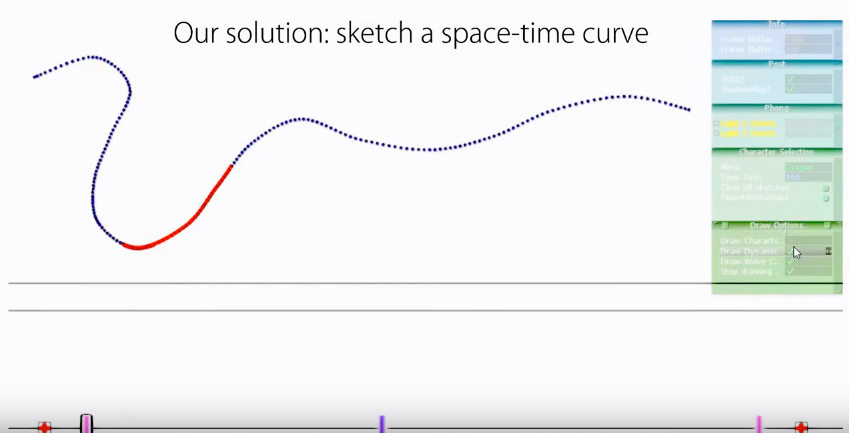
\includegraphics[scale=0.25]{spacetimecurve}
\caption{Drawing of INRIA's space-time curve}
\label{fig:spaceTimeCurve}
\end{figure}

Researchers in the IMAGINE group at INRIA (in Grenoble, France) have noticed this problem. They have made significant progress on a project called ERC Expressive, where they aim to offer more intuitive tools to author 3D digital content. The IMAGINE team has invented a technique for animation called space-time sketching, in which a user can draw a line in the path they want a model to take and it will be animated accordingly. As the character follows the path, its model bends and changes shape in a physically realistic way. Their system currently supports creating different movements with the path such as bouncing, rolling, and twisting.

\begin{figure}[!htb]
\minipage{0.32\textwidth}
  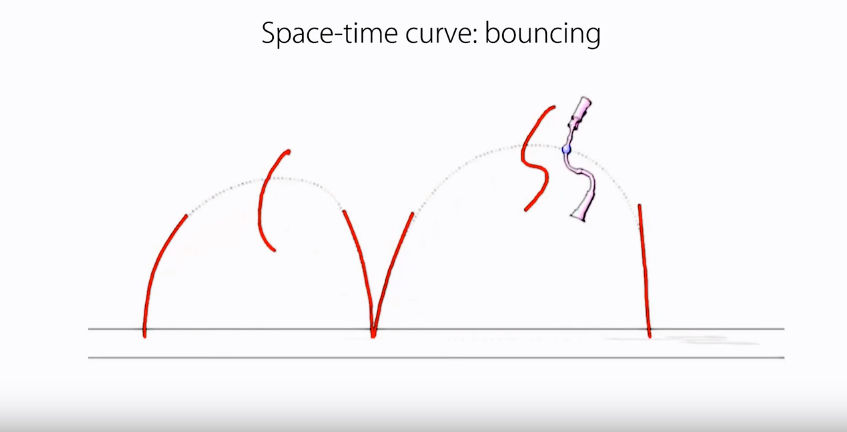
\includegraphics[width=\linewidth]{bouncing}
  \caption{Bouncing}\label{fig:bouncing}
\endminipage\hfill
\minipage{0.32\textwidth}
  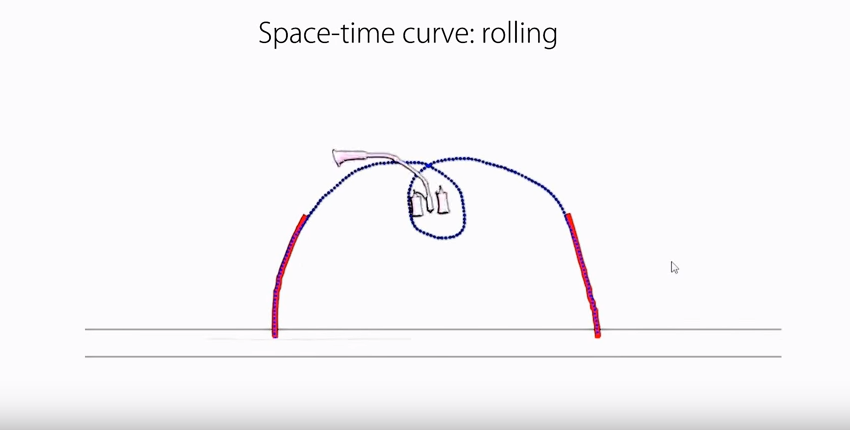
\includegraphics[width=\linewidth]{rolling}
  \caption{Rolling}\label{fig:rolling}
\endminipage\hfill
\minipage{0.32\textwidth}%
  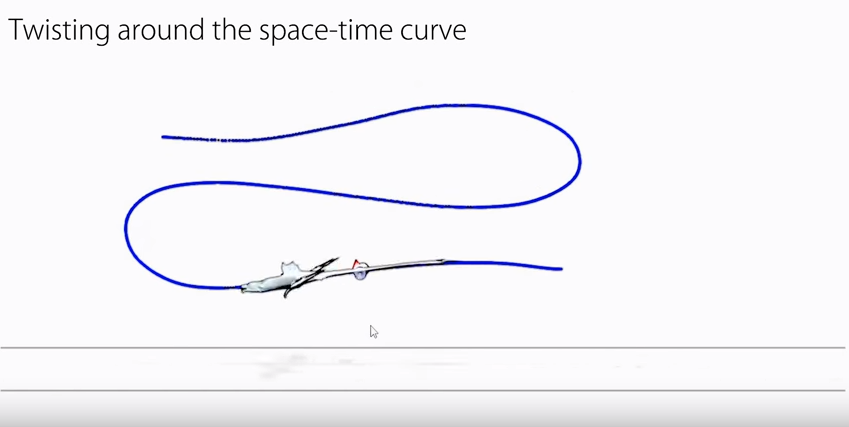
\includegraphics[width=\linewidth]{twisting}
  \caption{Twisting}\label{fig:twisting}
\endminipage
\end{figure}

Because IMAGINE's tool is a comprehensive system that has not yet been released, we want to develop a smaller version of this functionality within a plug-in for the game engine, Unity. One of the main goals of the IMAGINE team's research is to make animation more accessible to the general public. We share this goal, and want to narrow it down specifically to game developers. Many game developers (both amateur and professional) use Unity to make successful games, but some lack the artistic training to integrate high quality animations easily. Our plug-in aims to alleviate this task using INRIA's space-time sketching technique. 

We also want to allow for an animator to specify exceptions to the motions calculated by the algorithm so we will implement a variant of INRIA's technique. Our system will incorporate the notion of the ``default animation" for a shape, and be able to handle exceptions to it. For example, if a user wants to edit a motion they've made for a character, they will be able to specify a point on the drawn path where the motion will vary. To develop such an exception, we will take the original algorithm, recast it in  terms of constraint satisfaction in a non-monotonic language, and add enough apparatus to specify exceptions and deal with them.

\subsection{Features}
(See more in the Customer Requirements Document)
\begin{itemize}
 \item The user will be able to draw a line in 3D space from a selected object to its destination.
 \item The hand-drawn line will be used to calculate the motion and direction of the character, and then it will be animated.
 \item The animation generated should satisfy two constraints:
	\begin{itemize}
	  \item Be as close to the user-drawn line as possible
	  \item Be the most realistic animation possible based on the path
	\end{itemize}
 \item The user will be able to refine the path using control points and if time allows, editing of path can be done using the over-sketching technique.
 \item The user will be able to delete the paths they've drawn.
 \item The user will be able to see the paths they've drawn by selecting multiple characters at a time.
 \item If multiple characters have the same skeleton/rig (are copies of the same model), the user can copy and paste animations, by means of copying the paths, to other characters.
\item The user will be able to save and export paths to a file to be re-loaded into the plugin at a later time.
 \item This functionality will be presented in the form of a plugin to Unity.
\end{itemize}

\section{Statement of Work}
\label{sec:work}
\subsection{Unity UI prototypes}
Both prototypes will focus on drawing the path.

\subsubsection{Prototype \#1} 
\label{sec:ptype1}
The first prototype will be produced in order to help define requirements and provide the foundation for the full plugin. The features of the UI prototype will include the buttons, toolbar, panels, and tools needed to carry out what features we've described. This will help us identify potential requirements issues early on instead of later down the road. Based on the user's drawing motions, we will generate control points to form a path. We will create a simple toolbar which will feature a pen and mouse tool for drawing and refining the path, respectively. 

\subsubsection{Prototype \#2} 
\label{sec:ptype2}
Given an arbitrary set of control points, calculate and draw the B-spline in the viewport. The motivation for this prototype is to implement B-spline calculations for control points generated by user drawing on screen.

A few sets of control points will be predetermined and supplied as input for this prototype, so that this prototype is not completion dependent of the first prototype. However in practice the input of the B-spline calculator will be control points generated by the lines drawn by the user in the viewport.

The refining and deleting of the path are the next steps past the prototype and make up the UI functionality. This will be done with a separate refine path pen tool.

\subsection{Infrastructure setup}
This includes setting up the repository, automated build setup, and issue tracking software. Our repository of choice will be Github. We will also use Github to keep track of issues that arise during the development of our system. We shall also be using LaTeX to typeset the planning, requirement, and design documents as a standard which will be checked into Github and so we will be able to collaborate on it together and maintain revision history.

\subsection{UI Specifications}
Specifications relating to the Unity UI and how the user will use to engage with the core functionality. Our prototypes will be used to solidify the specifications. It will show us what can and cannot be done through the UI in the ways we have defined based on limited knowledge.

\subsubsection{Main canvas.} This will be the drawing area where paths are displayed as lines with square control points. Control points can be moved here using the Arrow tool. Paths can be drawn with the pen tool. Paths can be refined by drawing over / on top of already drawn paths using the path refine pen tool.

\subsubsection{Toolbar tray.} Located at the top of the window. This toolbar will contain an arrow tool, pen tool, and path refine pen tool.

\subsubsection{Path hierarchy palette.} This will include options to show/hide paths, show/fold subtrees and name/rename paths. Triangles will appear next to non-leaf node paths --- clicking on the triangle will show/hide the clicked path’s subtree.

\subsection{UI Test Plan}
The plan on how the UI will be tested and what criteria will correlate to successful implementation. As we go along making the first two prototypes, we can test the UI in phases based on what each prototype entails. The final phase of this testing will be User acceptance testing.

\subsection{UI Development}
A simple toolbar/tray will hold the pen and mouse tools. This toolbar can reside at the top of the interface window.

The main window will be the work area, where the paths can be drawn, and edited using the different tools available in the toolbar tray.

There will be a window to Show/Hide control paths for objects. Paths will be organized in a tree hierarchy. Each path may belong to any one parent path and have any number of child paths. This window will contain one path per line. Child paths will be indented one more indent unit than their parent. Parent paths can be folded such that their child paths are hidden. A triangle will appear to the left of any path that is not a leaf node. The triangle will point up when child paths are folded (hidden) and to the right when unfolded (visible). Paths can be renamed. The user can click the name, which will activate edit mode. Edit mode will use visual cues such as a border surrounding the path name with a contrasting background color. The user can click outside of this border box to exit edit mode or press the Escape or Enter/Return key.


\subsection{Core Functionality Specifications}
We will need to define the specifications relating to the core features of the project. As described later in the UI Development section, we have an initial idea of what we will need to do to implement our idea. After the prototype has been completed, we can go more into detail using the interface features and preliminary development work to show us what can, cannot, and still needs to be done. From there, we can make changes accordingly to the specifications. For example, we may find out through prototyping that the way we imagine the user drawing lines can't be done in Unity. Obviously we would have to modify that feature to fit both what we want and what is possible.

\subsection{Core Functionality Test Plan}
This plan will contain unit tests that need to be used in order to ensure all core functionality requirements are implemented correctly.

\subsection{Core Functionality Development}
Development of the core functionality. Break project development down into smaller pieces of the whole: UI frame (toolbars, tools, modes, buttons), UI functionality (path drawing, refining, copying), and core functionality (the animation generation, math). Develop and test each part independently, working toward finish from the ground up. Project can be stubbed out first with dummy methods.

\subsection{Challenges}
We have identified what we presume will be the most challenging parts of the project. Through our prototypes, we hope to demonstrate a preliminary use case: The user will be able to draw a 2D line that a 3D snake model will follow.

\subsubsection{3D Line Drawing}
The line drawing will be handled by the user interface. At first, we want to allow the user to draw a 2D line using the methods described in the statement of work. Then we will move on to 3D lines, which will include experimenting with ways the user can input the path information intuitively while maintaining precise functionality.
 
\subsubsection{General Algorithm}
In order to break down this task, we will first employ a simplified 2D version of it to very basic models (i.e. a snake). The path-following is the main goal. The secondary goal is to have the snake model itself bend (squash and stretch) according to the path and its physical constraints. Once this is working, we can generalize it to work with 3D lines in space and with more accuracy in terms of physical animation.

\subsubsection{Layering of Animations}
This will be tackled in the Winter term, since the previous two points must come before this in development. Once we have the line drawing and the algorithm working, we can begin work on blending animations by means of animation layers.


\section{Weekly Defect Reports}
During development a weekly report will be compiled that will include new defects and progress on existing defects. This is meant to be a tool to assist in timely defect resolution. Solutions to roadblocks and action items relating to defects can be addressed here.


\section{Product Manual}
A manual will need to be produced to assist users and explain the functionality of the product. This manual will contain everything that the user needs to know about how to successfully use our tool --- this might consist of what the UI will look like, how to use the UI, and output that the user can expect. 

This manual will also include a setup/installation manual to explain how the user can get started using our tool.


\subsection{Software}
\begin{itemize}
 \item Proper OS to develop Unity plugins (Windows or OSX)
 \item Student version of Unity
 \item Student version of Autodesk Maya
 \item Student version of Unreal Engine
\end{itemize}


\section{Resource List}
\label{sec:resource}
\subsection{Hardware}
Proper hardware and software is listed below to run Unity with best results:
\begin{itemize}
 \item Operating System: Windows XP SP2+, 7 SP1+, 8, 10, Mac OS X 10.8+
 \item GPU: Graphics card with DX9 (shader model 2.0) capabilities. Anything made since 2004 should work.
\end{itemize}


\section{Assumptions}
\label{sec:assumptions}
Users should have general knowledge of how to install Unity and how to navigate the software once executed.


\section{Schedule}
\label{sec:schedule}
Weeks marked with (F) denote finals week, and weeks marked with (H) denote holidays.

\subsection{Term 1}
Fall 2015 \\
What we will do and who will do it:
\begin{itemize}
	\item Define Project Plan - All, Lead: Sarah
	\item Define Customer Requirements - All
	\item Define Requirements Specification - All, Lead: Neil
	\item Begin Design Specification - All, Lead: Carlo
	\item Develop our two prototypes (This way, we can hopefully spot some expected problems noted in Section \ref{sec:risks} early on in the process.) - All, Lead: Angel \\
	The prototypes require:
	\begin{itemize} 
		\item UI icons - Sarah
		\item the GUI - Angel
		\item control points generation - Sarah, Carlo
		\item B-spline generation - Neil, Chris
	\end{itemize}
\end{itemize}

\begin{table}[H]
\centering
\begin{tabular}{|l|l|l|l|}
\hline
Week 	& Date	 		& Work	 		& 	Done?	 \\ \hline
1		& 09/21/15	 	& Form group		& 	yes		 \\ \hline
2		& 09/28/15	 	& Solidify idea	& 	yes		 \\ \hline
3		& 10/05/15	 	& Preliminary Plan document	& 	yes		 \\ \hline
4 (H)	& 10/12/15	 	& \specialcell{Fix plan document \\ and rethink project idea}	& 			yes \\ \hline
5		& 10/19/15	 	& \specialcell{Start Customer requirements document \\ and Start prototype \#1. See Section \ref{sec:ptype1} for details.}		& 			 \\ \hline
6		& 10/26/15	 	& \specialcell{Finish Customer requirements document \\ and work on prototype \#1}		& 			 \\ \hline
7		& 11/02/15	 	& \specialcell{Requirements specification \\ and work on prototype \#1} & 			 \\ \hline
8		& 11/09/15	 	& \specialcell{Requirements specification and Design \\and finish prototype \#1}		& 			 \\ \hline
9		& 11/16/15	 	& \specialcell{Design specification and Start \\ prototype \#2. See Section \ref{sec:ptype2} for details.}		& 			 \\ \hline
10 (H)	& 11/23/15	 	& \specialcell{Design specification \\ and work on prototype \#2}		& 			 \\ \hline
11		& 11/30/15	 	& Finish prototype \#2 development	& 			 \\ \hline
12 (F)	& 12/07/15	 	& Finalize Requirements		& 			 \\ \hline
\end{tabular}
\end{table}

\subsection{Term 2}
Winter 2016 \\
What we will do and who will do it:
\begin{itemize}
	\item Finalize Design Specification - All, Lead: Carlo
	\item Start core development, Unity is a priority - All, Lead: Angel
	\item Iteratively change Requirements and Design as needed based on Prototype - All, Leads: Neil, Carlo
	\item Determine if/how we can extend our product in the time remaining - All
	\item Release versions of product with limited functionality - All
	\item Begin Testing on completed features - All, Lead: Chris
\end{itemize}

\begin{table}[H]
\centering
\begin{tabular}{|l|l|l|l|}
\hline
Week 	& Date	 		& Work	 		& 	Done?	 \\ \hline
1		& 01/04/16	 	& Continue Design specification		& 			 \\ \hline
2		& 01/11/16	 	& \specialcell{Complete and Test Line Drawing  \\ capabilities in the prototypes}		& 			 \\ \hline
3 (H)	& 01/18/16	 	& Design specification and Start work on Line Refining		& 			 \\ \hline
4		& 01/25/16	 	& Test current UI features and Line Refining, Copying		& 			 \\ \hline
5		& 02/01/16	 	& Line Refining, Copying, Deleting		& 			 \\ \hline
6		& 02/08/16	 	& \specialcell{Finalize Design and change as needed \\ and Test Line capabilities}		& 			 \\ \hline
7		& 02/15/16	 	& Continue and finish Line capabilities		& 			 \\ \hline
8		& 02/22/16	 	& Start Animation Generation work		& 			 \\ \hline
9		& 02/29/16	 	& Continue Animation Generation work		& 			 \\ \hline
10		& 03/07/16	 	& Continue Animation Generation work			& 			 \\ \hline
11 (F)	& 03/14/16	 	& Continue Animation Generation work			& 			 \\ \hline
\end{tabular}
\end{table}

\subsection{Term 3}
Spring 2016 \\
What we will do and who will do it:
\begin{itemize}
	\item Continue and finalize Development - All, Lead: Angel, Animation math: Chris
	\item Develop extensions for Maya and Unreal, if time allows - All, Lead: Angel
	\item Continue and complete Testing on all features - All, Lead: Chris
	\item Prepare final release - All
\end{itemize}

\begin{table}[H]
\centering
\begin{tabular}{|l|l|l|l|}
\hline
Week 	& Date	 		& Work	 		& 	Done?	 \\ \hline
1		& 03/28/16	 	& \specialcell{Test current UI features and \\ Continue Animation Generation work	}	& 			 \\ \hline
2		& 04/04/16	 	& Continue Animation Generation work		& 			 \\ \hline
3		& 04/11/16	 	& Test current UI features		& 			 \\ \hline
4		& 04/18/16	 	& \specialcell{Assess what we can do in time remaining \\ and Test Animation Generation}		& 			 \\ \hline
5		& 04/25/16	 	& Test Animation Generation		& 			 \\ \hline
6		& 05/02/16	 	& Test Animation Generation		& 			 \\ \hline
7		& 05/09/16	 	& (tentative) Start Unreal port		& 			 \\ \hline
8		& 05/16/16	 	& Test all features and User Manual		& 			 \\ \hline
9		& 05/23/16	 	& Testing and User Manual		& 			 \\ \hline
10 (H)	& 05/30/16	 	& Final release		& 			 \\ \hline
11 (F)	& 06/06/16	 	& 		& 			 \\ \hline
\end{tabular}
\end{table}

\section{Risks}
\label{sec:risks}
\subsection{Schedule}
\begin{itemize}
 \item One or more parts of the project may not work as expected due to its complexity
 \item We may have delays due to unforeseen events
 \item Project gets rushed and some areas of the project get neglected
 \item Team members don’t have a set time to meet with the group
\end{itemize}

\subsection{Requirements}
\begin{itemize}
 \item Requirements may change unexpectedly
 \item Requirements are not fully known at the start of the project
 \item Some requirements may be neglected as a lower priority but in reality would be a higher priority
 \item Project’s target audience, focus, or goals change unexpectedly
\end{itemize}

\subsection{Technology}
\begin{itemize}
 \item Certain team members have little to no experience with animation which may lead to delays
 \item Editor/Development suite may be buggy and lead to delays
\end{itemize}

\subsection{Management}
\begin{itemize}
 \item Project doesn’t get reviewed often and we lose track of our progress
 \item Project members haven’t yet found out the constraints for each problem they might encounter
 \item One person assumes the role of multiple management roles
\end{itemize}

\subsection{Customer}
\begin{itemize}
 \item Customer might want to change the requirements unexpectedly in a major way
 \item Customer might want a change in the schedule which the team members can’t comply with
\end{itemize}

\section{Leaders}
This project is broken up into five different sections and each section has been designated a ``leader,” or somebody who is responsible for driving the completion of that section. The leaders for each section are listed below:
\begin{itemize}
 \item Project plan: Sarah Kushner
 \item Requirements: Neil Castelino
 \item Design: Carlo Rosati
 \item Development: Angel Delgado
 \item Testing: Chris Khedoo
\end{itemize}


\end{document}

